\subsection{Hard Probes of the Quark-Gluon Plasma}
\label{Sec:HardProbes}

High transverse momentum single hadrons, fully reconstructed jets,
open heavy flavor and heavy quarkonia provide information about the
strongly coupled QGP that complements the information provided by the
bulk and collective observables of the soft sector.  The higher
momentum and mass scales of these hard probes drive their production
to the earliest times in the collision; these same properties imply
that these probes don't completely thermalize during the evolution of
the produced medium.  The information imprinted on hard probes by QGP
production mechanisms and its later dynamics can therefore survive
into final state observables, making them uniquely valuable as
investigative tools of the complex emergent physics of the QGP.
However, accessing these very positive attributes of hard probes is
complicated in many cases by small production cross sections or the
need for specialized techniques and detectors.

In this section we first outline the future of jet studies over the
next decade, enabled by major developments in the RHIC and LHC
accelerator facilities and experiments described in
\ref{Sec:FacilitiesFuture}.  After that, we focus on the coming
prospects for open heavy flavor and heavy quarkonia measurements.

\subsubsection{Overview}

Previous studies at RHIC and the LHC have clearly demonstrated the ability 
to reconstruct jet observables in the high multiplicity heavy ion environment. 
Comparisons of hadronic and jet-based measurements to model calculations 
in a perturbative QCD framework have allowed the extraction of the QGP transport coefficient  \qhat\
with an uncertainty of about 50\%. Full jet 
measurements have demonstrated the modification of the dijet and photon-jet
momentum balance due to energy loss in the QGP, and have provided 
the first look at the modification of the jet structure itself due to 
interactions of the hard probe with the medium. These studies demonstrate the 
transport of energy from the jet core to low transverse momenta, close 
to thermal momentum scales, and away from the jet axis towards 
large angles far outside of the typical jet cone definition.

Future jet-based studies, built on the achievements at RHIC and the LHC, will 
address fundamental questions about the nature of QGP. These include 
precise measurements of QGP transport coefficients as a function of 
temperature, a detailed characterization of the QGP response to the 
parton energy loss and studies of the modification the jet angular 
and momentum structure as a function of angular and momentum scale. 
In combination, the goal of these studies is to determine the 
microscopic (or quasi-particle) nature of QGP 
and to understand how the macroscopic QGP liquid emerges from the 
underlying QCD degrees of freedom by probing the QGP dynamics over a wide range of length scales, see Figure\ \ref{Fig:HardProbesFuture} for a graphical representation.

This program will be enabled by the evolution of the RHIC and LHC 
accelerator facilities, upgrades to the existing experiments and the 
construction of sPHENIX, a state-of-the-art jet detector at RHIC. In 
parallel, experiment/theory collaborations will be strengthened 
and expanded, to fully utilize the increased precision and range of 
experimental observables. 

\begin{figure}[t]
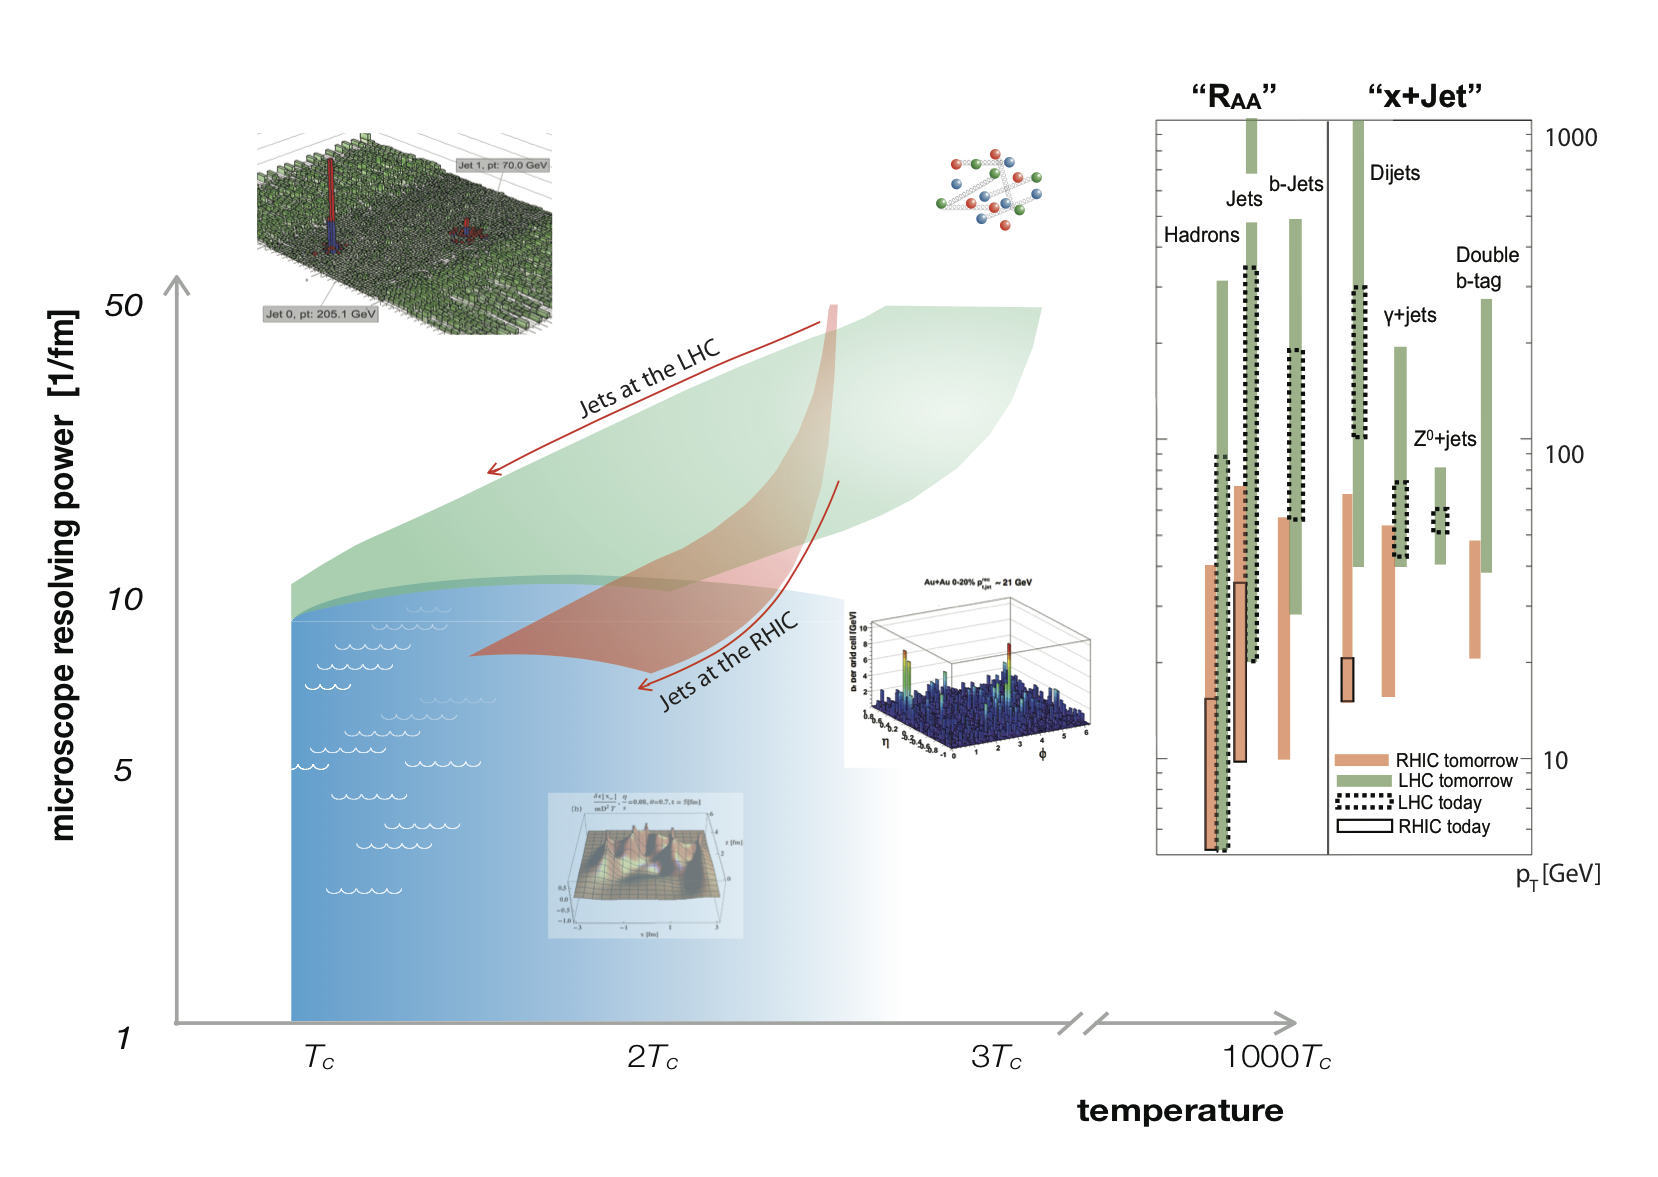
\includegraphics[width=1.05\textwidth]{fig/HardProbesFuture}
\caption[Graphical representation of a future physics goal]{Graphical representation of the future physics goal: Hard scattered partons at the LHC and at RHIC evolve through splittings and interaction with the medium, providing sensitivity to QGP dynamics over a wide range of length scales. The kinematic reach of future RHIC and LHC jet observables and their important kinematic overlap, enabled by new instrumentation at RHIC, is shown in an artist rendering.}
\label{Fig:HardProbesFuture}
\end{figure}

\subsubsection{Future jet physics capabilities at RHIC and LHC}
\label{Sec:FutureJetCapabilities}

Section~\ref{Sec:FacilitiesFuture} has provided an outline of the RHIC and LHC
accelerator and experiment upgrade plans. These upgrades benefit jet physics studies
at the two facilities in three major ways:
\begin{enumerate}
\item The statistical precision and kinematic reach for commonly used jet physics observables
is vastly increased, as shown in \ref{Fig:HardProbesFuture}). For single charged hadrons and reconstructed jets, the \pT\ reach will be 
extended by a factor of 2--3, up to 40~GeV for hadrons and 70~GeV for jets at RHIC (see Figure\ \ref{fig:AAphysics_projections}) and 
300~GeV and 1~TeV, respectively, at LHC. The increased lever arm will be crucial in further improving
the extraction of e.g.\ the \qhat\ coefficient from model comparisons. Equally importantly, 
the larger data sets will allow a more detailed determination of \qhat\ as a function
of path length and medium conditions, e.g.\ in very peripheral collisions in the two 
energy regimes.

\item Beyond increasing the kinematic range and statistical precision for 
current ``workhorse'' measurements, the combination of the increased luminosity at RHIC and LHC, 
increased LHC collision energy and the experiment upgrades will move 
the focus of experimental and theoretical studies to rare, highly specific
observables. Key examples are measurements of isolated photon + jet 
correlations at RHIC and LHC, as well as $Z^0$+jet correlations at LHC. 
As a benchmark, the number of recorded photon+jet events at LHC 
with $\ptg > 60$~GeV is expected to reach more than $3 \times 10^5$, compared
to about 3000 in the Run I data sets. Using the photon tag, the initial
energy of the scattered parton is determined on an event-by-event basis to about 15\%.
The photon tag also identifies the partons as quarks and provides their 
initial direction. Furthermore, the comparison of photon+jet events 
at RHIC and the LHC allows the selection of nearly identical initial 
hard scattering configurations embedded in different initial medium conditions
in terms of temperature and energy density (see Figure\ \ref{Fig:HardProbesFuture}). As jets and the medium co-evolve 
from their initial virtuality and conditions to final state hadrons, 
the comparison of various observables between the RHIC and LHC events
will provide key insights into the temperature dependence of the jet-medium
interactions. Future measurements enabled by this program include the 
absolute quark energy loss
as a function of quark energy and path length, modifications of the 
jet momentum and angular structure and the large angle momentum flow
and medium response as a function of event-by-event jet energy loss.
\item Finally, the very high statistics jet samples to be collected at the LHC and 
with a future state-of-the-art jet detector at RHIC will allow analyses based on 
a new generation of jet shape observables. There is intense activity
in the development of generalized jet structure variables at the LHC to maximize
the efficiency of discovery measurements by improving quark/gluon
discrimination and the tagging of boosted objects. Heavy ion studies 
of the modification of the jet momentum and angular structure through 
medium interactions will benefit greatly from these developments.
Present measurements at the LHC have shown the jet structure to be modified 
both within a typical jet cone size (e.g. $R = 0.5$) and beyond, with
the fragmentation products inside the cone shifted towards 
lower $\pt$ and larger angles and an associated transport of most of the ``lost''
jet energy outside of the typical jet cone size. First results 
at RHIC, probing different medium conditions, indicate similarities
in the modifications of the jet momentum structure, but possible
differences in the angular modifications. Using common, well-calibrated
jet shape observables at RHIC and the LHC in different regimes of 
medium conditions will be critical in relating the observed 
modifications to the fundamental properties of the QGP,
in extracting the temperature dependence of QGP transport coefficients
and ultimately in understanding the nature of the medium in the vicinity
of the phase transition and at temperatures much larger than $T_C$.

\end{enumerate}

\subsubsection{Future jet probes of the QGP}
\label{Sec:FutureJetProbes}

The combination of large increases in delivered luminosity over the next
decade, upgrades to the existing LHC detectors and the construction
of a state-of-the-art jet detector at RHIC will enable a coherent 
physics program employing well-calibrated common observables to
study jet modifications and jet-medium interactions over a wide 
range of medium conditions created at RHIC and the LHC, as shown
schematically in Figure\ \ref{Fig:HardProbesFuture}.
Together, RHIC and the LHC will provide a physics program that includes
a precision extraction
of QGP transport coefficients related to jet-medium interactions.
Even more importantly, this program will employ jets as a tool to understand how the 
observed strongly coupled (liquid) nature of the QGP arises from the 
underlying QCD micro-physics by probing the QGP dynamics over a wide range of length scales (see Figure\ \ref{Fig:HardProbesFuture}). 
By conducting these investigations we will move from observing what the properties
of QGP are to understanding how these properties 
arise from the underlying gauge theory.
%%%%%%%%%%%%%%%%%%%%
\pagebreak
%%%%%%%%%%%%%%%%%%%%

\begin{figure}
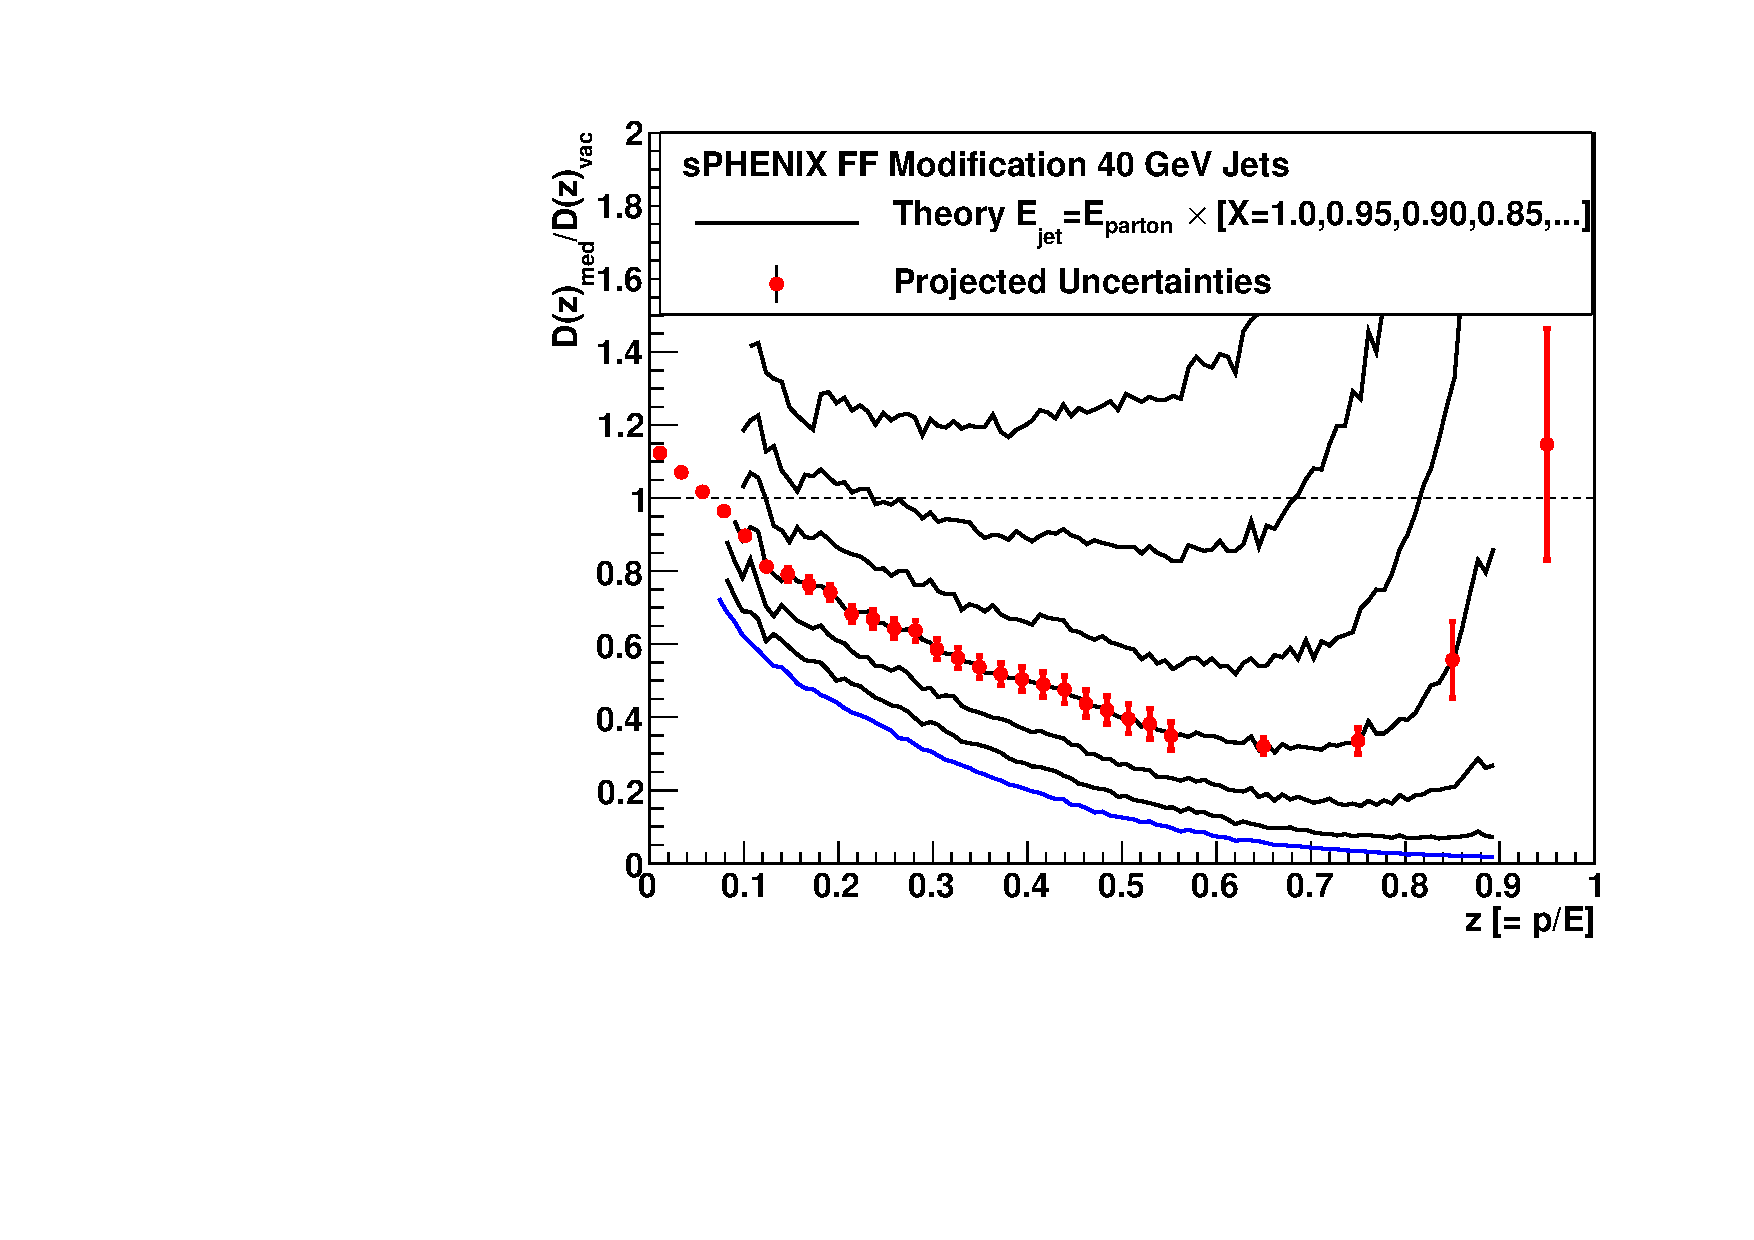
\includegraphics[width=0.9\textwidth]{fig/figure_ffmodification.pdf}
\caption[Projected sPHENIX statistical uncertainties on modified fragmentation functions]{Modified fragmentation function $D(z)$ in the medium\cite{Armesto:2007dt} expressed as the ratio of the modified $D(z)$ to that assuming vacuum fragmentation. The different black curves show the results of different assumptions for the fraction $X$ of the parton energy retained in the jet cone, with the original prediction corresponding to $X = 1.0$ shown as the lower blue curve. The projected statistical uncertainties are those achievable with sPHENIX for 22 weeks and 10 weeks of Au+Au and p+p data-taking, shown superimposed on the curve for $X = 0.85$. }
\label{Fig:sPHENIXfragfn}
\end{figure}
In detail, this future program includes:
\begin{enumerate}
\item Increased precision in extracting the average \qhat\ and \ehat\ 
transport coefficients, leading to a determination of their scale, energy and temperature dependence.
\item Combined global analysis of multiple observables at RHIC and the LHC 
to extract the temperature dependence of transport coefficients. Both
the RHIC and LHC final states represent an integral of jet-medium
interactions over the evolution of both the jet and the medium from initial
to final state. To disentangle the temperature dependence from
this evolution it will be essential to deploy directly comparable 
observables (theoretically and experimentally) in different 
QGP temperature regimes, in particular with respect to the fraction
of their evolution spend in the vicinity to the phase transition
region. Only a combined effort at RHIC and LHC can address this 
question.
\item Using increased systematic and statistical precision afforded
by new probes (e.g. photon-jet) to identity the medium response to
the modified jet radiation and further elucidate the liquid nature 
of the medium in its response to local perturbations
\item Using precision measurements of modifications of the jet structure 
in angular and momentum space to characterize the microscopic structure 
of the QGP. Jet probes here serve to perform experiments analogous to
Rutherford or deep-inelastic scattering off effective QGP constituents or 
quasi-particles. 
Perhaps the most straightforward signal is the modification of the 
jet fragmentation function $D(z)$, where $z = p/E$ is the momentum fraction 
of a single-particle of momentum $p$ in a jet of energy $E$. 
Other interesting observables include both potential modifications 
to the back-to-back jet scattering distributions, as well as modifications
of the intra-jet angular structure. For the latter, the correlated 
angular and momentum evolution of the jet from the initial scattering 
to the final hadronic structure probes probes a wide
range of scales, opening a window to interactions of jet 
and QGP constituents in between vacuum-like and in-medium cascade 
regimes. To pin down the physics of this intermediate window, 
systematic variations of both the jet conditions 
and medium conditions and dynamics are necessary. Combining RHIC and LHC 
measurements will allow control over initial density and temperature 
(in particular in respect to their vicinity to the critical temperature) 
and expansion dynamics of the system. The different energy regimes and 
tagging of particular initial states (photon+jet, $b$-tagged jets, 
multi-jet events) will allow selection of different or common 
jet populations in relation to different medium conditions. Success in 
this long-term endeavor will require a global analysis of 
a diverse set of RHIC and LHC data in an improved, well controlled
theoretical framework that makes explicit contact with the experimental observables.
\end{enumerate}


\subsubsection{Future challenges in the theory of jet modification}
\label{Sec:FutureJetTheoryChallenges}

In the period subsequent to the 2007 long range plan, there has been a major advance in the theoretical description 
of jet modifications in a dense medium. The ability of experiments both at RHIC and LHC to study full jet modification and 
energy flow with respect to the jet axis has led to the evolution from formalisms focused only on the leading particle towards full jet analyses tools.
Primarily, this has led to the ongoing development of several Monte-Carlo codes: YaJEM~\cite{Renk:2008pp,Renk:2010zx}, JEWEL~\cite{Zapp:2008gi}, MARTINI~\cite{Schenke:2009gb}, Q-PYTHIA~\cite{Armesto:2009fj}, PYQUEN~\cite{Lokhtin:2011qq}, and MATTER~\cite{Majumder:2013re}. While most of these routines are based on weak coupling, there is also a recently developed generator that is based on a hybrid strong and weak coupling approach~\cite{Casalderrey-Solana:2014bpa}. 

All of these approaches are based on one of the established analytical formalisms, and as such, apply to slightly different epochs in the lifespan of a hard jet in a dense medium. As a jet emanates from a hard interaction, it is far off its mass shell, at such hard scales that the jet probes the medium at extremely short distances characterized by its high-$Q^{2}$ 
structure of a dilute gas of partons. In this regime, it is expected that the parton's interactions with the medium are
dominated by radiation of gluons over elastic scattering processes.  
As the virtuality of the partons within a jet begins to drop, different parts of the jet enter different regimes.
The very energetic jet fragments undergo several scatterings per emission in which the multiple scattering prevents their virtuality from falling
below $\hat{q} \tau$, where $\tau$ is the lifetime of 
the parton.
As a result, those hard partons remain weakly coupled with the medium. 
The less energetic partons in the shower decrease in virtuality to the scale of the medium 
(of the order of the local temperature) and become strongly coupled. 
Currently most of the Monte Carlo descriptions apply to only one of these regimes, under the assumption that such a regime dominates the measured observables (with varying approximations regarding the medium). 
Nonetheless, several of these event generators have been tested against a variety of observables, 
such as jet $R_{AA}$,
dijet energy and angular imbalance, 
intra-jet hadron distribution and jet shapes~\cite{Renk:2013rla,Renk:2012cb,Ramos:2014mba,Zapp:2012ak,Young:2012dv,Majumder:2013re}. 
One of the outstanding challenges in this field will be the development of a generator that smoothly interpolates between the various regimes of jet quenching while incorporating a fluctuating medium simulated by an event-by-event viscous fluid dynamical simulation. This will be followed by rigorous testing and validation against all available 
jet data. 


Full jet reconstruction, however, involves more than simply a perturbative redistribution of the energy within a jet cone.
Rather, as the energy is deposited within an evolving medium it thermalizes and forms a source of energy and momentum current for the fluid dynamical evolution of the medium. 
A significant fraction of the this energy is carried away from the jet at large angles, with the remainder found 
within the reconstructed jet cone. To date only initial efforts have been made to understand the dynamics of energy deposition and redistribution 
within a fluid medium~\cite{Neufeld:2009ep,Qin:2009uh}, and this remains an open issue. 
In addition to this question of energy redistribution at the medium scale, another outstanding question is the distribution of radiation at the perturbative scale. The ordering of radiation from a hard parton in vacuum is well established, however its modification in the medium is still an open question. There now exist two separate calculations, one in the radiation dominated regime~\cite{Fickinger:2013xwa} which shows no ordering, and one in the 
scattering dominated regime~\cite{Armesto:2011ir}, which shows anti-angular ordering. A resolution of these issues at NLO remains one of the major opportunities in the theory of 
pQCD energy loss. It may indeed turn out that a full understanding of this problem leads to the development of an effective theory of jet modification in dense matter. To date, 
great strides have been made in modifying Soft Collinear Effective Theory (SCET)~\cite{Bauer:2000yr,Bauer:2001yt,Bauer:2002nz} by the addition of off-shell gluon modes with momenta transverse to the collinear modes within a hard jet. 
This modified version of SCET has been uses to calculate the 
propagation, scattering and emission from hard partons in a dense medium~\cite{Idilbi:2008vm, DEramo:2010ak,Ovanesyan:2011xy}. Extending this beyond the radiation dominated regime to the multiple scattering regime remains a future goal. Several model calculations~\cite{CasalderreySolana:2011rq,Qin:2010mn} have already laid the groundwork for what a fully developed jet modification theory should look like. 


Developing in parallel with the theoretical description of parton showers in a dense medium is the improved description of transport coefficients, which are the actual measurable quantities that describe the medium probed by hard jets. A great deal of work has gone into determining the temperature dependence of the transverse diffusion coefficient $\hat{q}$. 
More recently, efforts have been made to determine the longitudinal energy loss coefficient $\hat{e}$. 
While light flavor energy loss is known to be weakly dependent on $\hat{e}$, this is not the case for 
heavy flavors. 
Significant theoretical activity now focuses on determining the dynamics of heavy flavor energy loss 
and the sensitivity of these and other heavy flavor observables
to $\hat{e}$~\cite{Qin:2009gw,Djordjevic:2013pba,Abir:2014sxa}. 
Efforts to extend this to $b-$tagged jets are also being carried out~\cite{Huang:2013vaa}. 
Future developments in the theory of heavy flavor dynamics in the medium serve not only as a consistency check for the pQCD based formalism of jet modification, but also provide the 
primary means to determine the drag coefficient $\hat{e}$.

While the dependencies of the transport coefficients on temperature reveal the dynamics of the medium as seen by the jet, they also depend on the scale and energy of the jet. 
Recently there has been a series of developments to quantify this scale and energy dependence of transport coefficients by carrying out NLO calculations of these coefficients, 
most notably of $\hat{q}$. Several calculations, once again performed in different regimes of jet quenching, have obtained rather different dependencies on energy and 
scale~\cite{Liou:2013qya,Kang:2013raa,Blaizot:2014bha,Iancu:2014kga}. Much theoretical effort is currently being devoted to a resolution of these differences. 
In all of the current jet quenching calculations, either of leading particles or of full jets, the normalization of the transport coefficients is determined
empirically by fitting to one data set. 
%This situation will remain 
%even after all issues with renormalization have been settled.
While this emphasizes the absolute requirement of parallel theoretical and experimental investigations,
it also demonstrates that the current calculations of jet modifications do not result directly from the QCD Lagrangian. In an effort to 
resolve this, several groups have considered the possibility of evaluating such coefficients 
on the lattice~\cite{Majumder:2012sh,Panero:2013pla,Ji:2013dva}. These represent 
extremely difficult calculations which, however, hold the promise of determining the transport coefficients with no input other than the local temperature. 
Future calculations of transport coefficients on the lattice, combined with calculations of the 
scale and energy dependence described above will allow for a rigorous and first principles test of the entire formalism of jet modification.



\subsubsection{Future Quarkonia measurements at RHIC and the LHC}
\label{Sec:FutureQuarkonia}

%\begin{figure}[!pht]
%   \centering
%   \begin{subfigure}[b]{0.72\textwidth}
%      \includegraphics[width=0.9\textwidth]{fig/upsilon_mass_subtracted_0_10pc_10Bevts}
%       \caption{The di-electron invariant mass distribution  for 0--10\% central \AuAu\ events after 
%                      the combinatorial background has been removed by subtracting all like-sign pairs.}
%        \label{Fig:upsilon_auau_0-10pc}
%    \end{subfigure}
%    
%    \begin{subfigure}[b]{0.72\textwidth}
%        \includegraphics[width=0.9\textwidth]{fig/upsilon_raa_10pc_bins_100Bevts}
%        \caption{ Estimate of the statistical precision of a measurement of the
%                       $\Upsilon$ states assuming that the measured $R_{AA}$ is equal to the results of a recent theory
%                      calculation~\cite{Strickland:2011aa} }
%         \label{Fig:upsilon_raa}
%    \end{subfigure}
%
%    \caption{Projected quarkonia results from a 10 week \AuAu\ run with sPHENIX.}
%\end{figure}

\begin{figure}[!pht]
  \centering
      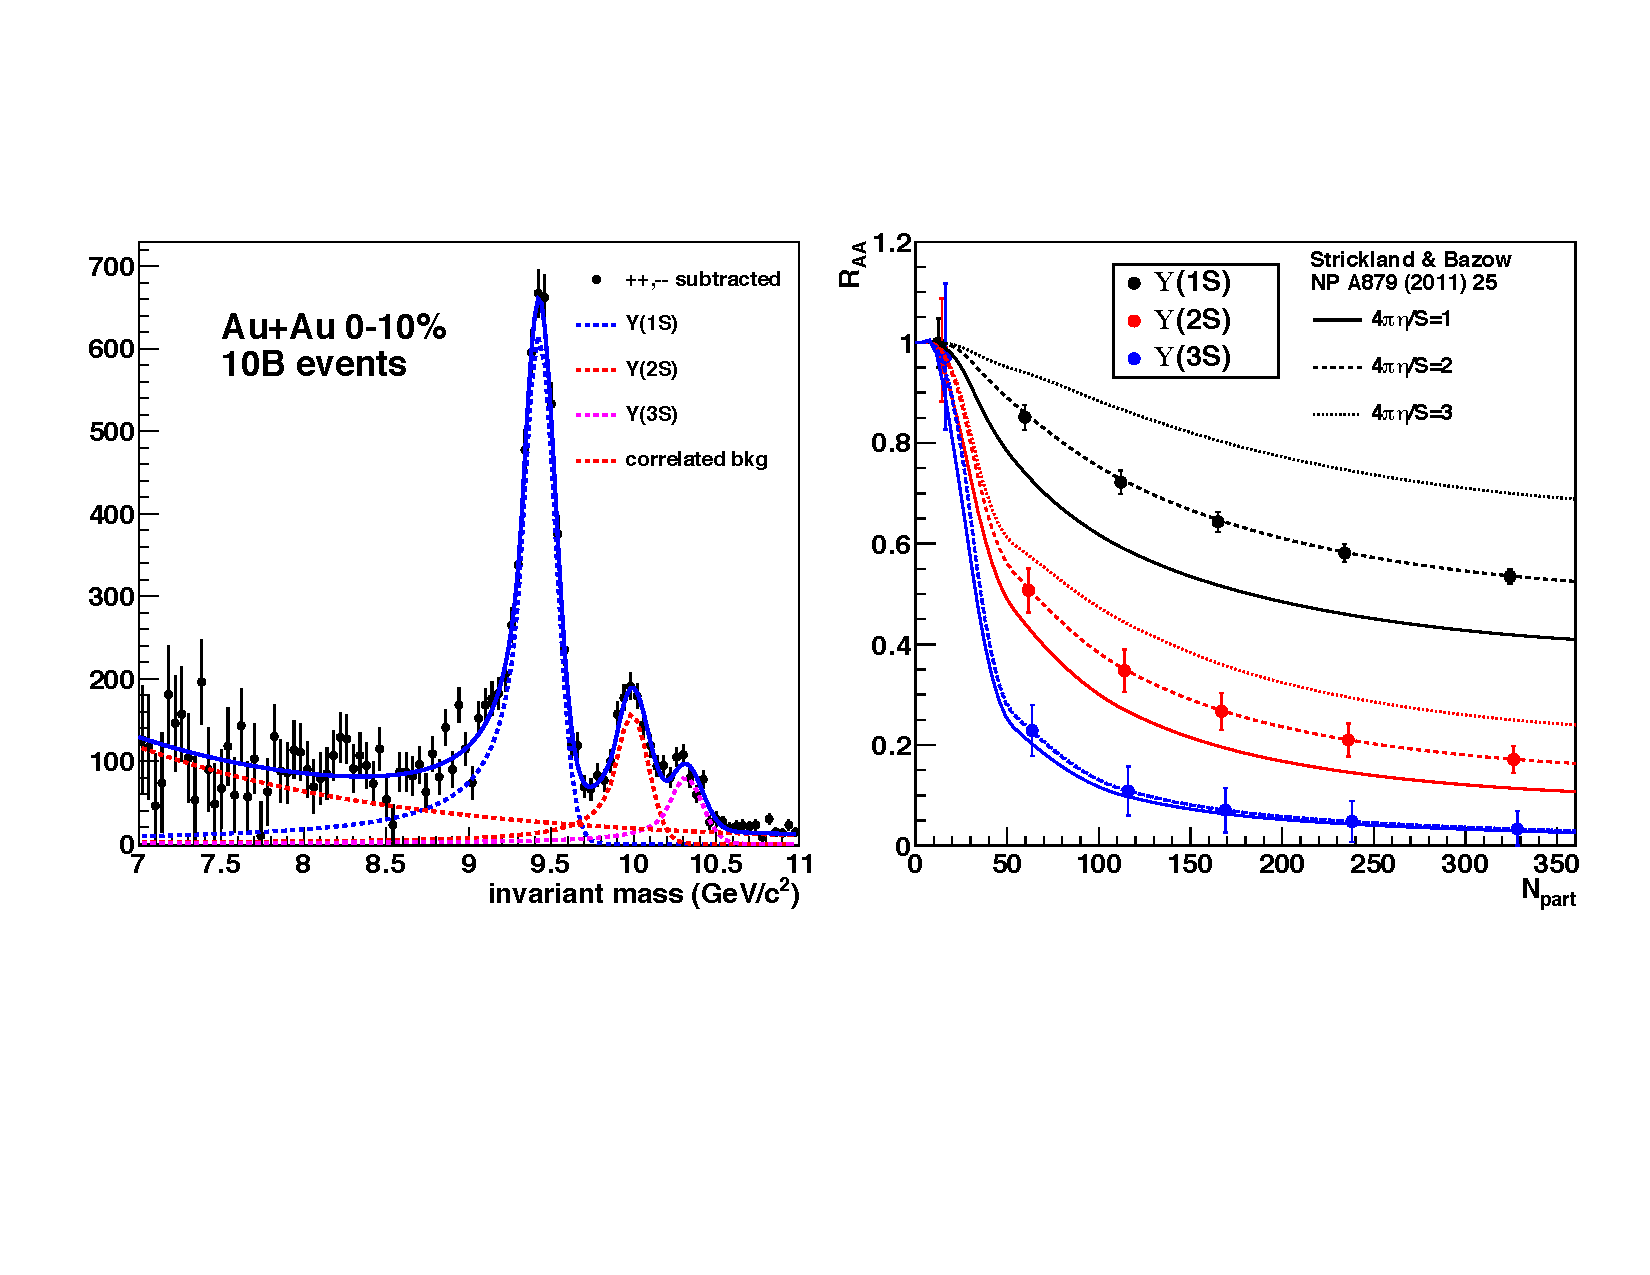
\includegraphics[width=\textwidth]{fig/upsilon_combined}
      \caption[Projected quarkonia results from a 20 week \AuAu\ run
        with sPHENIX]{Projected quarkonia results from a 20 week \AuAu\ run
        with sPHENIX.  (left) The di-electron invariant mass
        distribution for 0--10\% central \AuAu\ events after the
        combinatorial background has been removed by subtracting all
        like-sign pairs. (right) Estimate of the statistical
        precision of a measurement of the $\Upsilon$ states assuming
        that the measured $R_{AA}$ is equal to the results of a
        recent theory calculation~\cite{Strickland:2011aa}.}
\label{Fig:upsilon_auau_0-10pc}
\label{Fig:upsilon_raa}
\end{figure}

In addition to the jet capabilities added at RHIC by the sPHENIX detector upgrade, 
outlined in Section~\ref{Sec:FacilitiesFuture}, high precision
measurements of the modification of the $\Upsilon(1S)$, $\Upsilon(2S)$ and $\Upsilon(3S)$
states in A+A and $p$+A collisions will also be provided by sPHENIX. The key features 
of the upgrade that enable this are:

\begin{itemize}

\item The 1.5 T magnetic field of the Babar magnet, combined with precise tracking, will 
provide 100 MeV mass resolution for measurements of $\Upsilon \rightarrow e^+e^-$ decays
at mid rapidity.

\item Good signal to background performance is obtained by using low mass tracking to limit 
radiative losses for electron tracks and the Electromagnetic and Hadronic calorimeters to 
reject combinatoric background from charged hadrons.

\item Increased RHIC luminosity combined with the large acceptance of sPHENIX
and long RHIC running times provide the statistical precision for the $\Upsilon$ measurements at RHIC that will
tightly constrain theoretical models of the modification. These measurements will 
complement similar high precision measurements at higher temperature from LHC 
experiments that will be available on a similar time scale (i.e. by the end of LHC Run 3) 
due to LHC machine and detector upgrades, and accumulated luminosity.

\end{itemize}

Critical variables to manipulate when probing the QGP are the temperature of
the QGP and the length scale probed in the medium. For this reason, measurements 
at two widely different temperatures of the three Upsilon states, which span a large range of 
binding energies and sizes, are ideal. However for comparisons between data at RHIC and the LHC
 to be effective, high precision is required at both facilities.

The planned program of measurements at RHIC starting in 2021 includes \pp\,
\pAu\ and \AuAu\ measurements. A very important feature for $\Upsilon$ 
measurements with sPHENIX is that the increases in \pp\ luminosity at RHIC will permit a
measurement of the \pp\ reference cross section having similar precision to that which can be
attained in \AuAu\ and \pAu\ collisions. The projected invariant mass spectrum for central collisions
from a 10 week \AuAu\ run is shown in Figure~\ref{Fig:upsilon_auau_0-10pc}. This spectrum is shown
after the combinatorial background has been subtracted, and assumes no modification of the yields relative
to \pp\ collisions. 


The projected statistical precision for measuring the nuclear suppression factor $R_{AA}$ in a 20 week \AuAu\ run, using \pp\
reference data also from a 10 week run, is illustrated in Figure~\ref{Fig:upsilon_raa}. 
For the sake of this illustration it is assumed that the suppression for each state
is equal to that from a theory calculation~\cite{Strickland:2011aa} in which the shear viscosity to
entropy density ratio is a parameter. The data are expected to provide good constraints on models.

At the LHC, CMS has measured the $\Upsilon$ modification in $\sqrt{s_{NN}}$=2.76 GeV Pb+Pb
collisions with mass resolution that cleanly resolves the three states. It is expected that CMS will 
accumulate (at $\sqrt{s_{NN}}$=5.5 TeV) by the end of Run 3 an $\Upsilon$ data set that is roughly 
100 times larger than their existing one, yielding statistical precision that is even better than that expected 
from sPHENIX. 

The different color screening environments caused by the different temperatures attained in collisions at RHIC 
and LHC, combined with large differences in the time evolution of the QGP and in the underlying bottom
production rates, make them distinctly different laboratories for studying the effect of the plasma on the 
$\Upsilon$ states. The combination of high precision $\Upsilon$ data from the LHC and RHIC will 
constrain theoretical models in ways that data measured at only one energy could not.